% Attempting to convert solutions to docx and then go from there.

\documentclass[lang=en]{skrapport}
\nonstopmode
\usepackage[utf8]{inputenc}
\usepackage{graphicx}
\usepackage{amsmath,amssymb}
\usepackage[ocgcolorlinks]{hyperref}
\usepackage{tabularx}
\usepackage{booktabs}
%\usepackage[american,siunitx]{circuitikz}
%\newcommand{\equal}{=}
\usepackage{float}
\usepackage{siunitx}
\usepackage{enumitem}
\usepackage{tikz}
\usepackage{bodegraph}
\begin{document}
	
	% See Nillseon Textbook.
\paragraph{Problem 1}

The bandpass filter was originally designed for $Q > 20$ with $R = 5 \ k\Omega$, $L = 2 H$ and $C = 50 pF$. Now the filter is loaded with $R_L$, but the quality factor is not to drop below 10. What is the smallest possible value of the load resistor $R_L$, given the transfer function.
\begin{figure}
	\centering
	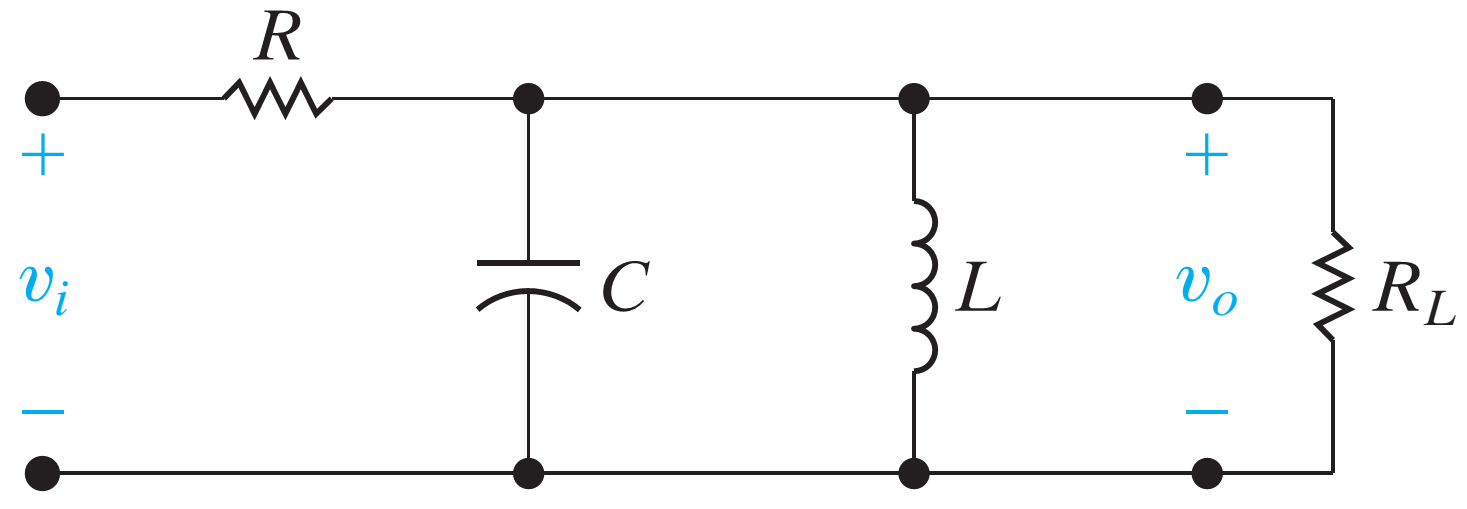
\includegraphics[width=1\linewidth]{question1.png}
	\caption{Question 14-34}
	\label{fig:question1}
\end{figure}
\[
H(\omega)=\frac{v_o(\omega)}{v_i(\omega)}=\cfrac{j \omega L / R}{1+J\omega L \left(\frac{1}{R}+\frac{1}{R_L}\right) + (j \omega)^2 LC}
\]
\begin{align*}
& \omega_0 = \frac{1}{\sqrt{LC}} = \frac{1}{\sqrt{2 \times 10^{-6}}}
\end{align*}
\end{document}